\documentclass{standalone}
\usepackage{tikz}
\usepackage{ctex,siunitx}
\usepackage{tkz-euclide}
\usepackage{amsmath}
\usetikzlibrary{patterns, calc}
\usetikzlibrary {decorations.pathmorphing, decorations.pathreplacing, decorations.shapes,}
\begin{document}
\small
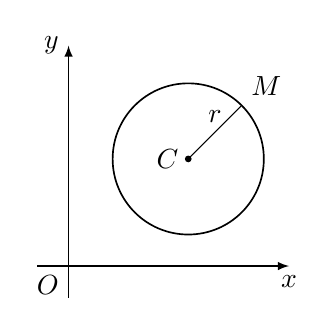
\begin{tikzpicture}[>=latex,scale=0.8]
  \draw[thin,->](-0.5,0)--(3.5,0)node[below]{$x$};
  \draw[thin,->](0,-0.5)--(0,3.5)node[left]{$y$};
  \tkzDefPoints{0/0/O,1.9/1.7/C}
  \draw[semithick](C)circle(1.2);
  \tkzDrawPoints[fill=black](C)
  \draw(C)--++(45:1.2)node[midway,above]{$r$};
  \node at ([shift=(45:1.2)]C)[above right]{$M$};
  \tkzLabelPoints[below left](O)
  \tkzLabelPoints[left](C)
\end{tikzpicture}
\end{document}